\section{Simulations}

\subsection{Implementation notes}
All the results presented in the following sections were obtained with the implementation of an RK4 method of integration either with constant or varying timesteps. The constant timesteps method is a straightforward implementation of RK4 with 4 calculations of positions with each step. The varying timesteps method is adaptative and accepts a step only if an RK4 step and two RK4 steps with $\Delta / 2$ are closer than a tolerance $\varepsilon$ in meters. If not it reduces $\Delta t$ until this condition is verified. It can also increase $\Delta t$ to allow for larger steps when only small errors arise.

% For the adaptative time steps scheme a choice had to be made when division by 0 were encountered. Some simulations gave a value of $d=0$ i.e.
% \begin{verbatim}
% y1 = RK4_do_onestep(x, t, dt);
% y_tilde = RK4_do_onestep(x, t, dt / 2.0l);
% y2 = RK4_do_onestep(y_tilde, t, dt / 2.0l);
% \end{verbatim}
% gave the same values for y1 and y2. To avoid a division by 0 in the next step of increasing the dt as such
% \begin{verbatim}
% dt = dt * pow(tol / d, 1.0l / (4.0l + 1.0l));
% \end{verbatim}
% a condition (d != 0.0l) was added before this calculation. If (d==0) the dt is kept constant.

\subsection{Transfer orbit}
The first simulations were about simulating the transfer of Webb from a low Earth orbit ar $r_0$ to the L2 Lagrange point at $r_1$ as defined in \autoref{sec:transfer_anal}. The system was initialised with \(r_0 = 6800\) km and the value of $v0$ calculated using \autoref{eq:v0_final}. Using the third Kepler law the predicted orbit was of duration $t_\mathrm{fin} = 2\pi\sqrt{a^3/Gm_T}$ and the simulation was run up to $t_\mathrm{fin}/2$. The results for the fixed $\Delta t$ scheme with $n_\mathrm{steps} = 5000$ and for an adaptative scheme with tolerance $\varepsilon = 100$ \si{\meter} are shown in \autoref{fig:transfert_traj}. The adaptative scheme obtained the given trajectory in $n_\mathrm{steps} = 65$.
\begin{figure}[h]
    \centering
    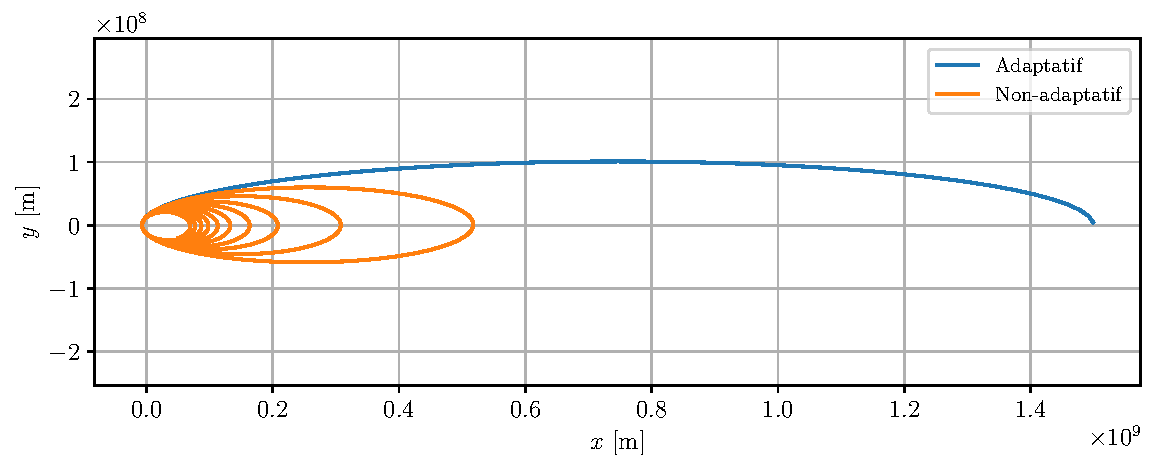
\includegraphics[width=\linewidth]{figures/transfert_comparaison.pdf}
    \caption{Trajectories of a transfer orbit from $r_0 = 6800$ \si{\kilo\meter} to the L2 Lagrange point at $r_1 = 1.5 \cdot 10^6$ \si{\kilo\meter} with varying (adaptative), tolerance $\varepsilon = 100$ \si{\meter}, and constant (non-adaptative) timesteps, $n_\mathrm{steps} = 5000$}
    \label{fig:transfert_traj}
\end{figure}

The \autoref{fig:transfert_traj} shows clearly that the fixed $\Delta t$ scheme is not adaptated to simulating these orbits with the trajectory not reaching the expected point L2 from the theory by a long distance. We see this method doing multiple orbits during the time it should have taken to complete only one. The adaptative scheme conversely gives exactly the expected behavior with the simulation ending extremely close to the theoretical L2 point representing half of the orbit.

The energies of these two simulations were also analysed and the results are shown in \autoref{fig:transfert_energies}. The \autoref{fig:transfert_2_energies} shows that the energy was highly not conserved for the non-adaptative method with a loss of more than $5\cdot10^6$ \si{\joule}. This corresponds to what was expected from the trajectories in \autoref{fig:transfert_traj} with the energy decreasing with the lowering orbits. Compared to the non-adaptative method, the method with varying $\Delta t$ had a seemingly constant energy. However a more precise plot shows in \autoref{fig:transfert_adapt_energy} that the energy did drop by $\sim 200$ \si{\joule} at the very beginning of the simulation. This corresponds to the point in the orbit where it was closest to the Earth and thus with the most errors. For the rest of the simulation the energy was very well conserved with this method.
\begin{figure}[h]
    \centering
    \begin{subfigure}{0.47\linewidth}
        \centering
        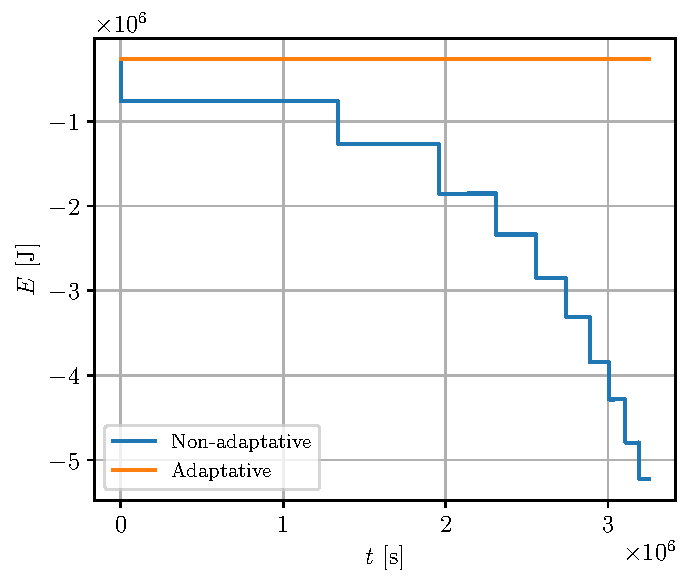
\includegraphics[width=\linewidth]{figures/transfert_all_energy.pdf}
        \caption{Constant and varying $\Delta t$}
        \label{fig:transfert_2_energies}
    \end{subfigure}
    \begin{subfigure}{0.52\linewidth}
        \centering
        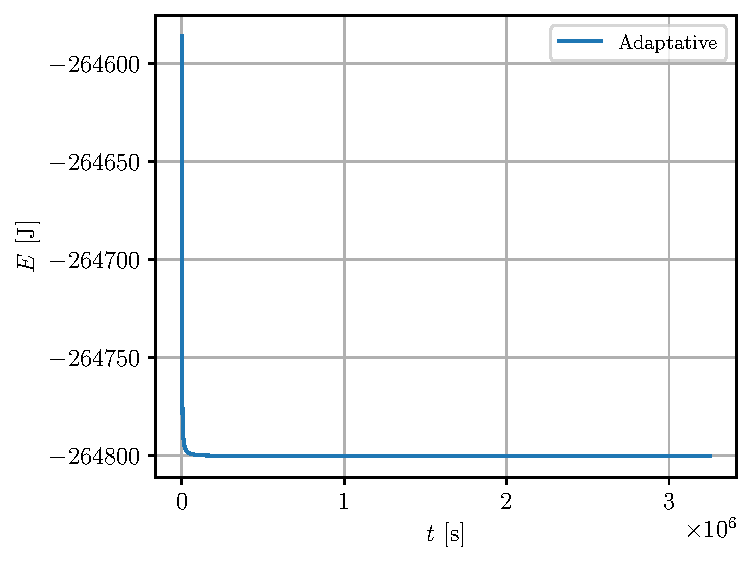
\includegraphics[width=\linewidth]{figures/transfert_adapt_energy.pdf}
        \caption{Varying $\Delta t$}
        \label{fig:transfert_adapt_energy}
    \end{subfigure}
    \caption{Energies during the simulation up to $t_\mathrm{fin}/2$ for two numerical methods}
    \label{fig:transfert_energies}
\end{figure}

The results of these two simulations indicate clearly that the adaptative RK4 method gives much better results in this simulation of an orbit of transfer than the RK4 method with constant $\Delta t$. The energy was conserved better and the behavior of this adaptative method was as expected for low computation costs, of only 65 timesteps even if those steps require more operations.

\subsection{Orders of convergence}
The convergence of these two methods was also analysed to determine if they behaved similarly and as expected when $\Delta t \to 0$. The convergence for the position and energy are illustrated in \autoref{fig:transfert_errors}. To simulate higher $n_\mathrm{steps}$ for the adaptative methods the tolerance $\varepsilon$ was decreased so that the steps would need to be smaller to achieve the required condition. The error on the position was directly calculated knowing the final theoretical position $\vec{r}_\mathrm{th} = \left(r_1, 0, 0\right)$. It is clearly illustrated in \autoref{fig:transfert_error_pos} that the convergence is of order 4 for both the adaptative and non-adaptative RK4 methods for the position. The error on the conservation of energy was calculated using the difference between the maximum and the minimum of the energy throughout the simulation. The results in \autoref{fig:transfert_error_energy} show that the order of convergence is again 4 for both methods. Thus the Runge-Kutta order 4 method does converge in order 4 for this problem of transfer orbit and with both constant and adaptative timesteps.

\begin{figure}[h]
    \centering
    \begin{subfigure}{0.49\linewidth}
        \centering
        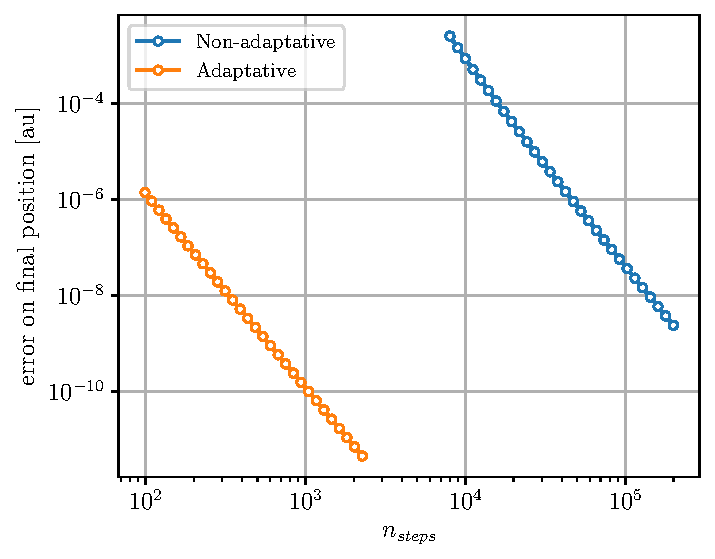
\includegraphics[width=\linewidth]{figures/transfert_error_pos.pdf}
        \caption{Error on position}
        \label{fig:transfert_error_pos}
    \end{subfigure}
    \begin{subfigure}{0.49\linewidth}
        \centering
        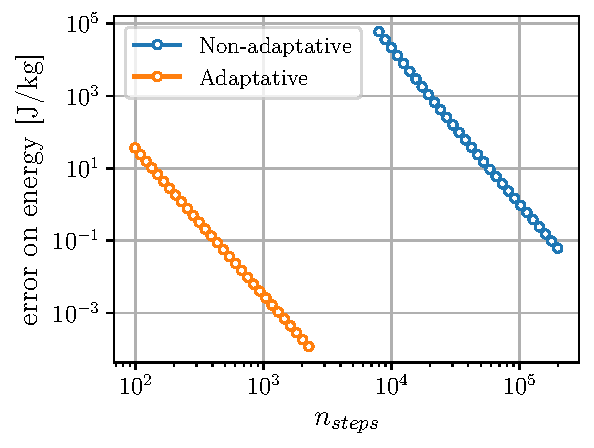
\includegraphics[width=\linewidth]{figures/transfert_error_energy.pdf}
        \caption{Error on conservation of energy}
        \label{fig:transfert_error_energy}
    \end{subfigure}
    \caption{Convergence of errors on position and energy conservation for the adapative and non-adaptative RK4 methods}
    \label{fig:transfert_errors}
\end{figure}

A final result of this error analysis is that even if the order of convergence is the same for both methods the errors are significantly different. For both the position and the energy 200 steps of the adaptative method give the same final errors as with 200.000 steps of the constant $\Delta t$ method. This difference of 3 orders of magnitude of steps for similar errors is again an indicator that the adaptative method is very well suited to this type of orbital mechanics problems.

\subsection{Around Lagrange L2}

We now consider the reduced 3-body problem, like in \ref{sec:3body_reduced}. The simulations are done in the \(\mathcal R'\) reference frame, placing Webb at the Lagrange L2 point given in \ref{sec:lagrange_L2} and giving the satellite an initial downwards speed \(\dot y' = -0.1\) m/s. In this sections, the simulations are done until \(t_\textrm{fin} = 2\) years. The trajectory of the satellite is given in \autoref{fig:lagrange_trajectory} and will be discussed later. We will first analyse the convergence of both methods.

Due to the nature of the adaptative timestep method, the convergence order against \(\frac{1}{n_\textrm{steps}}\) will be analysed. The results wit the initial conditions given above are reported in \autoref{fig:lagrange_conv}. Both methods converge with order 5 to \(x' \approx 0.999771678\) au and \(y' \approx -0.004537985\) au, which was obtained using a linear fit. While the convergence order is the same, the adaptative method gets close to the final position for a much smaller amount of steps: the rightmost point on \autoref{fig:lagrange_conv_adapt} corresponds to a \(n_\textrm{steps} < 2000\) while being more precise than the rightmost point on \autoref{fig:lagrange_conv_fixed}, which had \(n_\textrm{steps} = 10000\).

\begin{figure}[h]
    \centering
    \begin{subfigure}{0.45\linewidth}
        \centering
        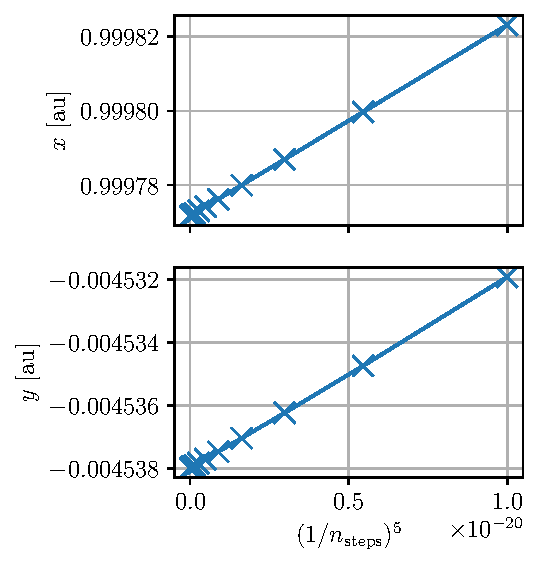
\includegraphics[width=\linewidth]{figures/lagrange_convergence_fixed.pdf}
        \caption{Fixed \(\dd t\) method}
        \label{fig:lagrange_conv_fixed}
    \end{subfigure}
    \begin{subfigure}{0.49\linewidth}
        \centering
        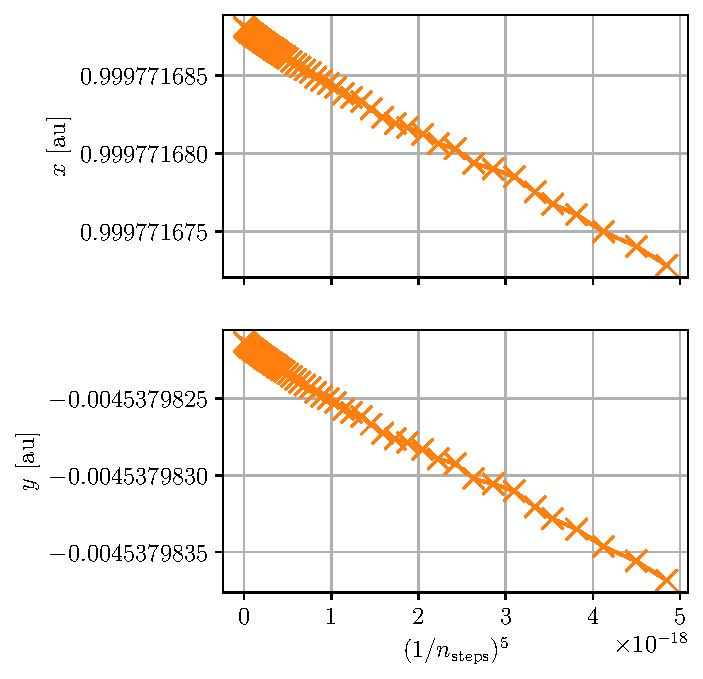
\includegraphics[width=\linewidth]{figures/lagrange_convergence_adapt.pdf}
        \caption{Adaptative \(\dd t\) method}
        \label{fig:lagrange_conv_adapt}
    \end{subfigure}
    \caption{Final position convergence starting from L2 with initial downwards speed \(\dot y' = -0.1\) m/s for both methods. \(n_\textrm{steps}\) was varied from \(10^4\) to \(10^6\) for the fixed timestep method and the tolerance \(\varepsilon\) was varied from \(10^{-5}\) to \(10^{-1}\) for the adaptative method.}
    \label{fig:lagrange_conv}
\end{figure}

Mechanical energy over time is shown in \autoref{fig:lagrange_emec}. Both methods seem to give similar energy levels. Error on conservation of mechanical energy for both methods is also given in \autoref{fig:lagrange_emec_error}. While both methods give a similar error, the initial spread is much smaller for adaptative method than the fixed one. While mechanical energy does not seem to be conserved well for each step, mechanical energy seems to recover after each bump, making it a bit more conserved overall. Analysing the location of the spikes in energy reveals that they occur at the intersection between the trajectory and the Earth-Sun axis (\(x'\) axis). This is shown in \autoref{fig:lagrange_max_mins_energy}. These locations corresponds to brutal changes in speed along the \(y'\) axis.

\begin{figure}[h]
    \centering
    \begin{minipage}{.45\textwidth}
        \centering
        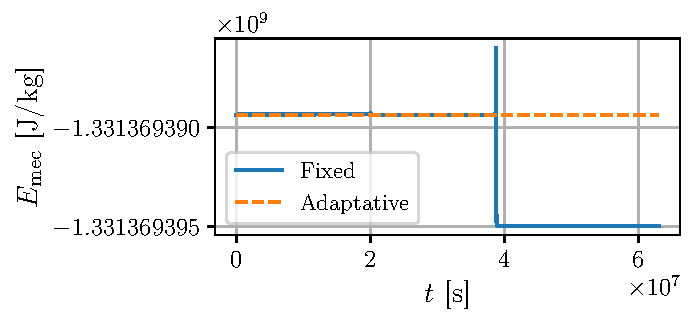
\includegraphics[width=\linewidth]{figures/lagrange_emec.pdf}
        \captionof{figure}{Mechanical energy over time for both methods}
        \label{fig:lagrange_emec}
    \end{minipage}
    \hspace*{1cm}
    \begin{minipage}{.45\textwidth}
        \centering
        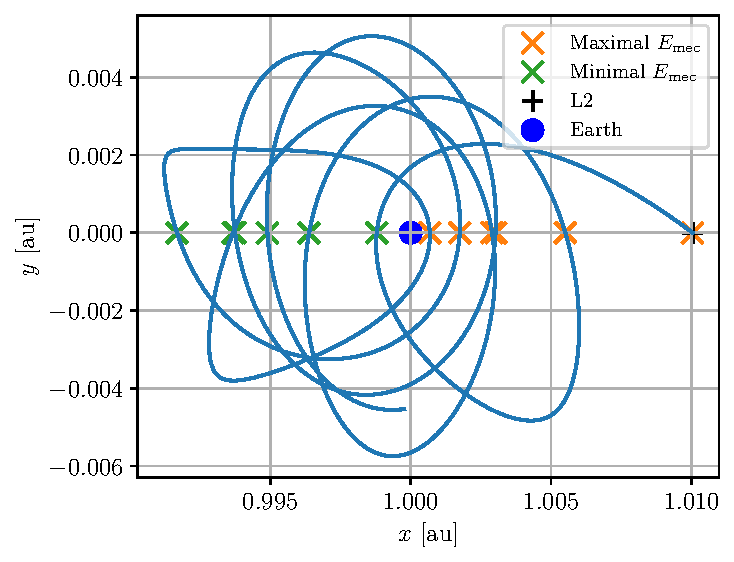
\includegraphics[width=\linewidth]{figures/lagrange_max_mins_energy.pdf}
        \captionof{figure}{Points on trajectory where mechanical energy is maximal or minimal, using adaptative method}
        \label{fig:lagrange_max_mins_energy}
    \end{minipage}
\end{figure}

\begin{figure}[h]
    \centering
    \begin{subfigure}{0.48\linewidth}
        \centering
        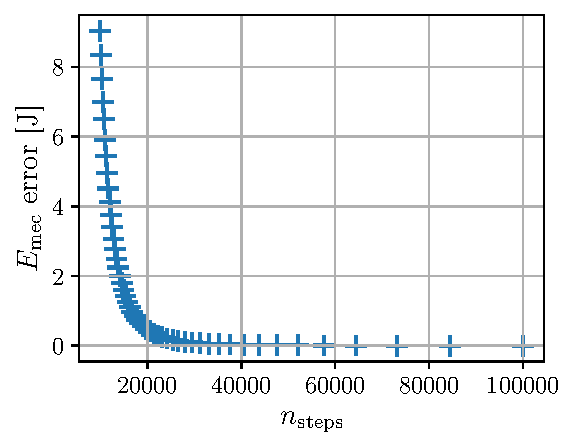
\includegraphics[width=\linewidth]{figures/lagrange_emec_error_fixed.pdf}
        \caption{Fixed \(\dd t\) method}
        \label{fig:lagrange_emec_error_fixed}
    \end{subfigure}
    \begin{subfigure}{0.48\linewidth}
        \centering
        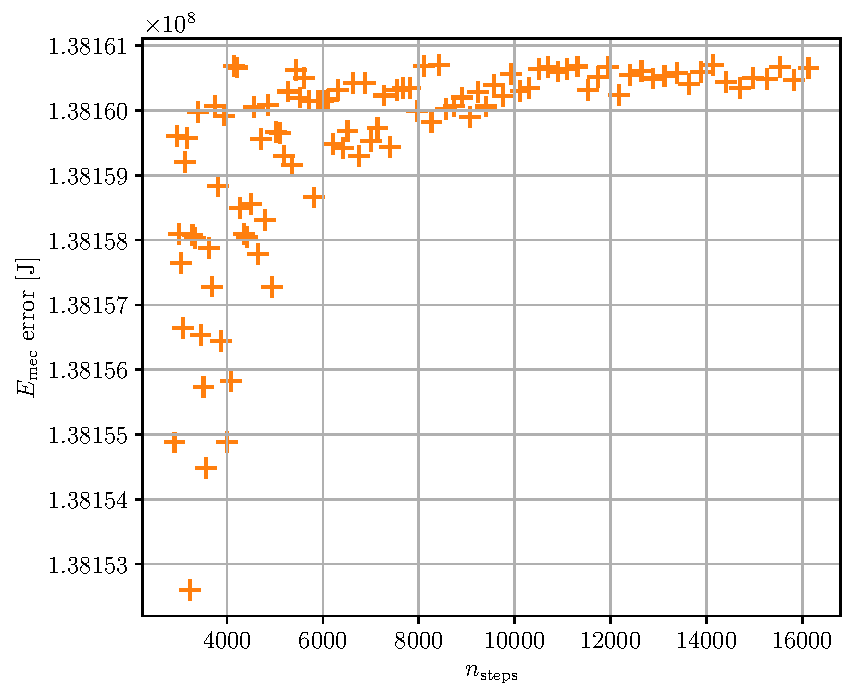
\includegraphics[width=\linewidth]{figures/lagrange_emec_error_adapt.pdf}
        \caption{Adaptative \(\dd t\) method}
        \label{fig:lagrange_emec_error_adapt}
    \end{subfigure}
    \caption{Mechanical energy error starting from L2 with initial downwards speed \(\dot y' = -0.1\) m/s for both methods. \(n_\textrm{steps}\) was varied from \(10^4\) to \(10^6\) for the fixed timestep method and the tolerance \(\varepsilon\) was varied from \(10^{-5}\) to \(10^{-1}\) for the adaptative method.}
    \label{fig:lagrange_emec_error}
\end{figure}

Let's analyse the trajectory more closely, specially the behavior near L2. Using the initial configuration given at the beginning of this section, we get the trajectory given in \autoref{fig:lagrange_trajectory}. Because of the initial perturbation, the satellite falls towards Earth and starts orbiting. It gets trapped in the potential field of the Earth, as is clearly shown in \autoref{fig:lagrange_trajectory_potential}. This result is expected because the Lagrange point L2 is unstable, as will be discussed later. The small downwards speed reduces the centrifugal force, which pushed the satellite away from Earth. A lower centrifugal force thus means that the satellite gets pulled towards Earth. If the initial speed was upwards, the satellite would get pushed away! The trajectory in \autoref{fig:lagrange_v0_up} shows this.

\begin{figure}[h]
    \centering
    \begin{subfigure}{0.46\linewidth}
        \centering
        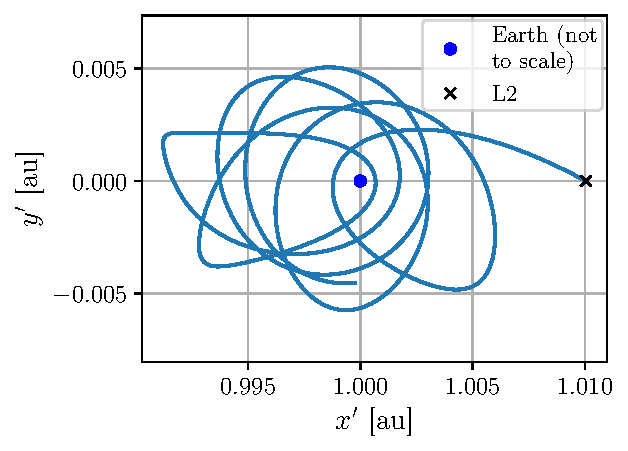
\includegraphics[width=\linewidth]{figures/lagrange_trajectory.pdf}
        \caption{Trajectory using adaptative method}
        \label{fig:lagrange_trajectory}
    \end{subfigure}
    \begin{subfigure}{0.53\linewidth}
        \centering
        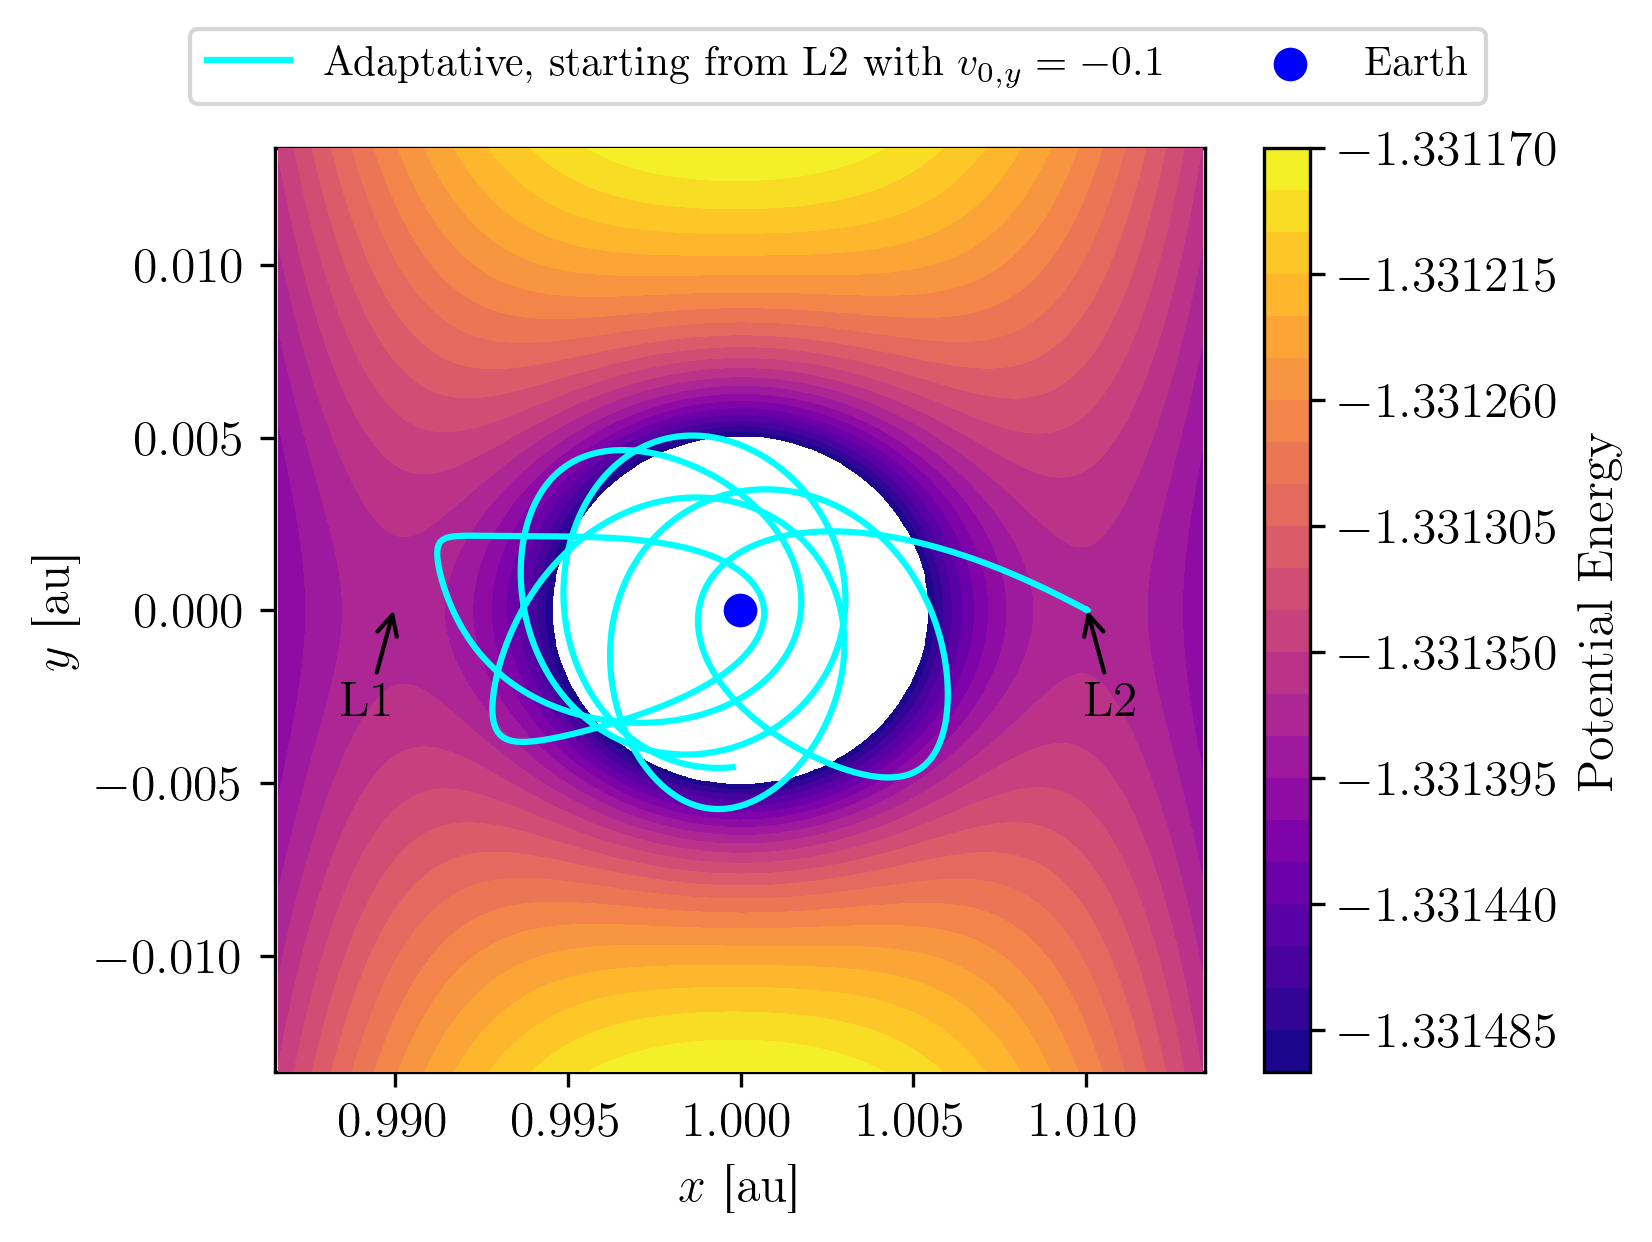
\includegraphics[width=\linewidth]{figures/potential_L1_L2_zoom_trajectory.png}
        \caption{Trajectory with potential}
        \label{fig:lagrange_trajectory_potential}
    \end{subfigure}
    \caption{Trajectory of Webb after falling in the potential well of the Earth}
\end{figure}

\begin{figure}[h]
    \centering
    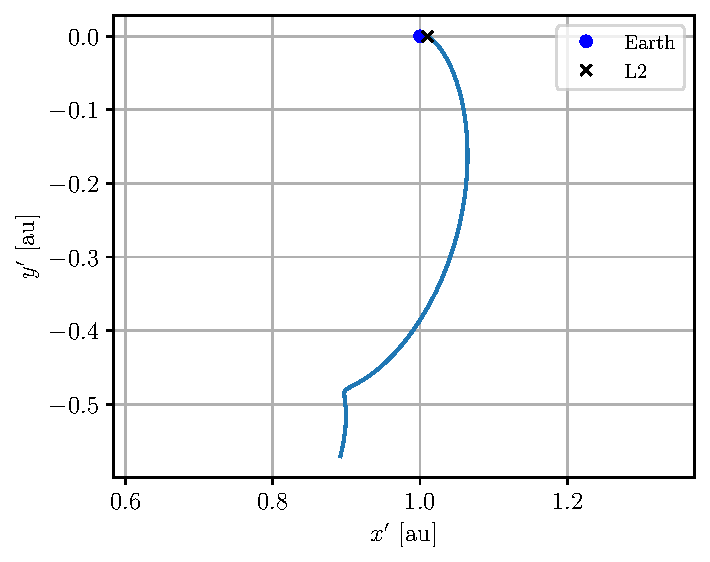
\includegraphics[width=0.6\linewidth]{figures/lagrange_v0_up.pdf}
    \caption{Trajectory starting from L2 with initial upwards speed \(\dot y' = 0.1\) m/s, using adaptative method with tolerance \(\varepsilon = 10^{-4}\)}
    \label{fig:lagrange_v0_up}
\end{figure}

It is interesting to note that the distance to L2 grows exponentially over time, for a given range. Indeed, \autoref{fig:lagrange_distance_L2} shows that this range is for \(t < 2 \cdot 10^7 \textrm{ s} \approx 231 \textrm{ days}\), after which the satellite remains far from L2.

\begin{figure}[h]
    \centering
    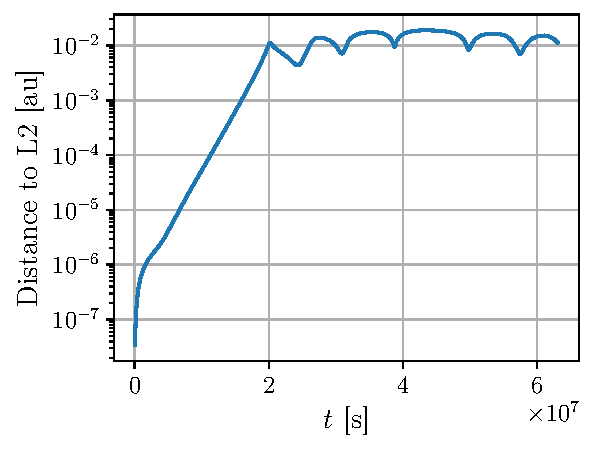
\includegraphics[width=0.6\linewidth]{figures/lagrange_exponential_distance.pdf}
    \caption{Distance from L2 over time, starting from L2 with initial downwards speed \(\dot y' = -0.1\)}
    \label{fig:lagrange_distance_L2}
\end{figure}

Let's study the potential energy a bit more closely, allowing us to find the stability of the Lagrange point L2 for example. At the scale of the solar system, we can identify a bump in the potential, which could hint at the presence of other Lagrange points. There is a ring where potential increases slightly, as shown in \autoref{fig:lagrange_potential_global}. While the scale of the figure does not show it, there should be saddle points and some wells allowing for other Lagrange points, whose locations are marked approximately on the figure \cite{lagrange}. Around the Earth, it is possible to see that the Lagrange points L1 and L2 are placed on saddle points, meaning they are unstable. \autoref{fig:lagrange_L1_L2}. This is coherent with what was observed in the simulations. Another visualisation of the potential is shown in \autoref{fig:lagrange_potential_3D}.

\begin{figure}[h]
    \centering
    \begin{subfigure}{0.48\linewidth}
        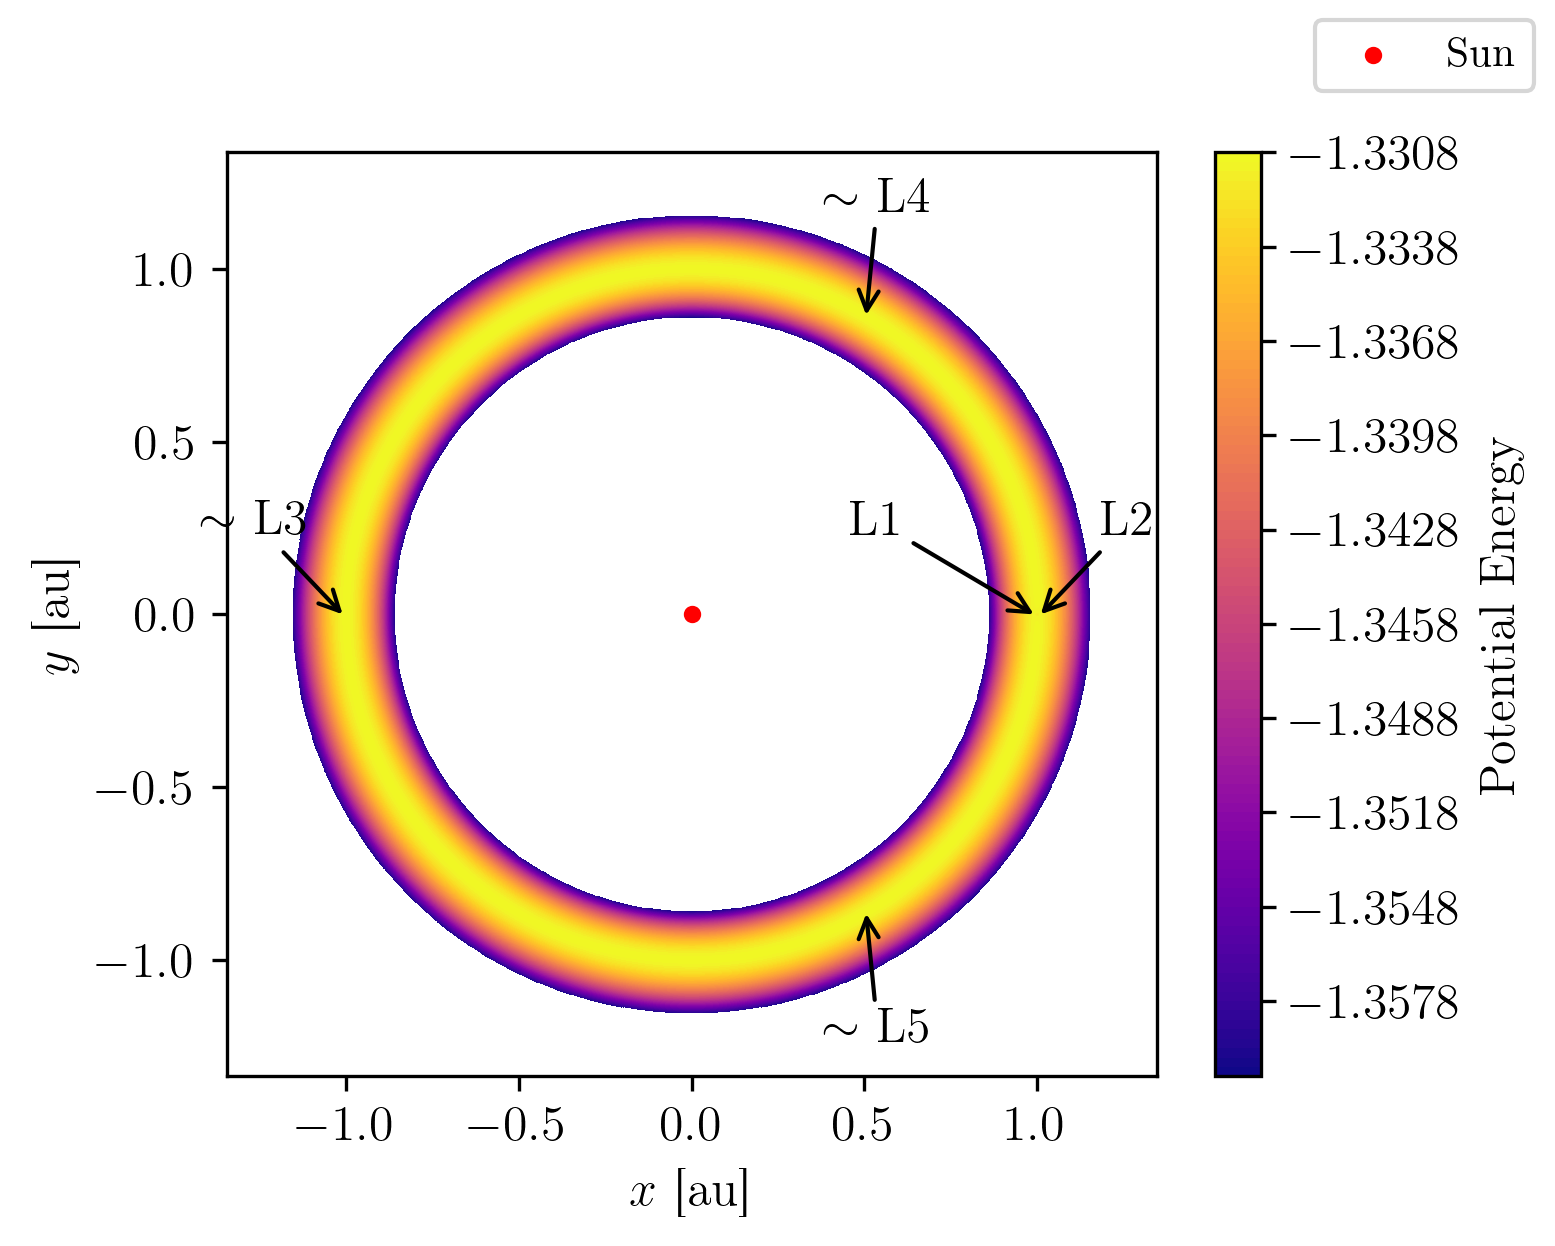
\includegraphics[width=\linewidth]{figures/potential_global.png}
        \caption{Potential energy band for a distance around the Sun-Earth distance.}
        \label{fig:lagrange_potential_global}
    \end{subfigure}
    \begin{subfigure}{0.48\linewidth}
        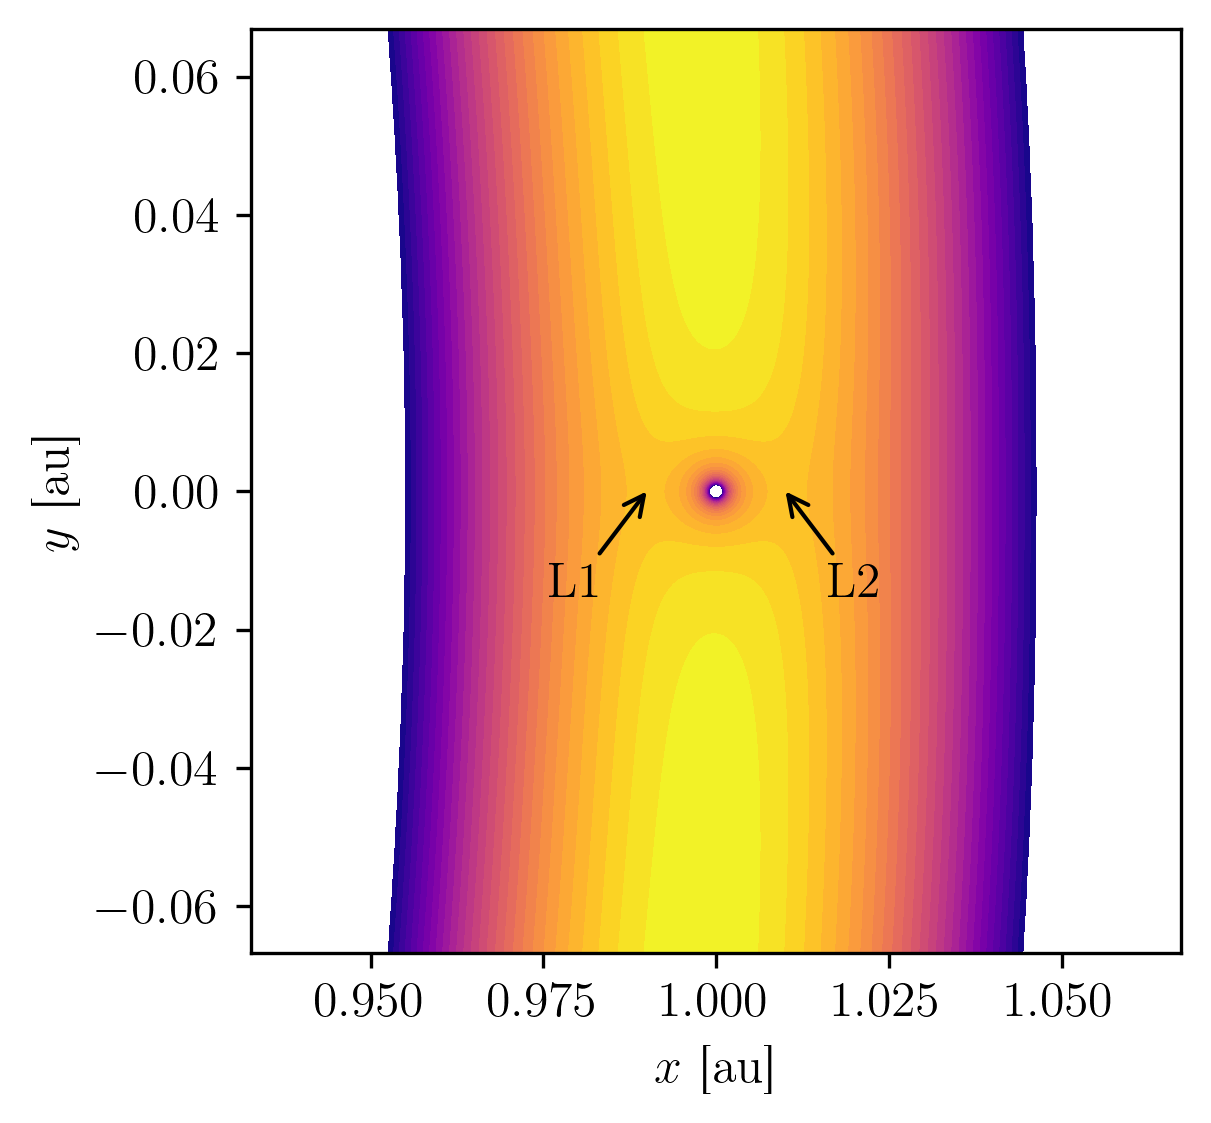
\includegraphics[width=\linewidth]{figures/potential_L1_L2_zoom.png}
        \vspace*{0.2cm}
        \caption{Potential energy around Earth}
        \label{fig:lagrange_L1_L2}
    \end{subfigure}
    \caption{Potential energy at different points in the Sun-Earth system}
\end{figure}

\begin{figure}[h]
    \centering
    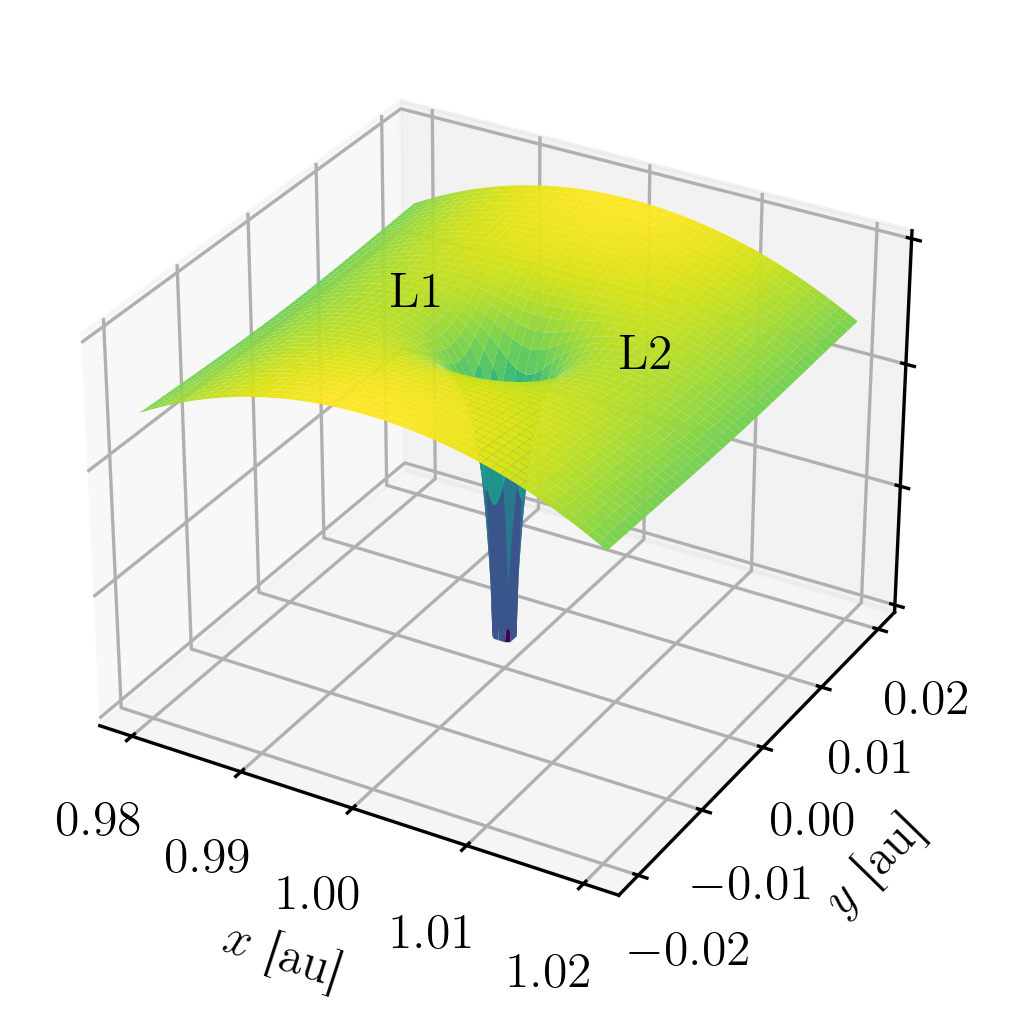
\includegraphics[width=0.6\linewidth]{figures/potential3D_L1_L2_zoom.png}
    \caption{3D representation of the potential around Earth}
    \label{fig:lagrange_potential_3D}
\end{figure}